\setlength{\columnsep}{3pt}
\begin{flushleft}
\bigskip

\paragraph{nmcli command}

\begin{itemize}
	\item nmcli stands for \textbf{network manager command line}.
	\item It is a command-line tool for controlling NetworkManager.
	\item nmcli save configuration files in the \textbf{/etc/sysconfig/network-scripts} directory.
	\item Using \textbf{"nmcli"} command, you can assign/change IP address to network interface card.
	\item Options with \textbf{nmcli} command:
	\begin{itemize}
		\item Display all available LAN card devices:
		\begin{tcolorbox}[breakable,notitle,boxrule=-0pt,colback=pink,colframe=pink]
			\color{black}
			\fontdimen2\font=9pt
			Syntax: nmcli device show
			\newline
			or
			\newline
			Syntax: nmcli dev show
			\fontdimen2\font=4pt
		\end{tcolorbox}
		Eg:
		\begin{figure}[h!]
			\centering
			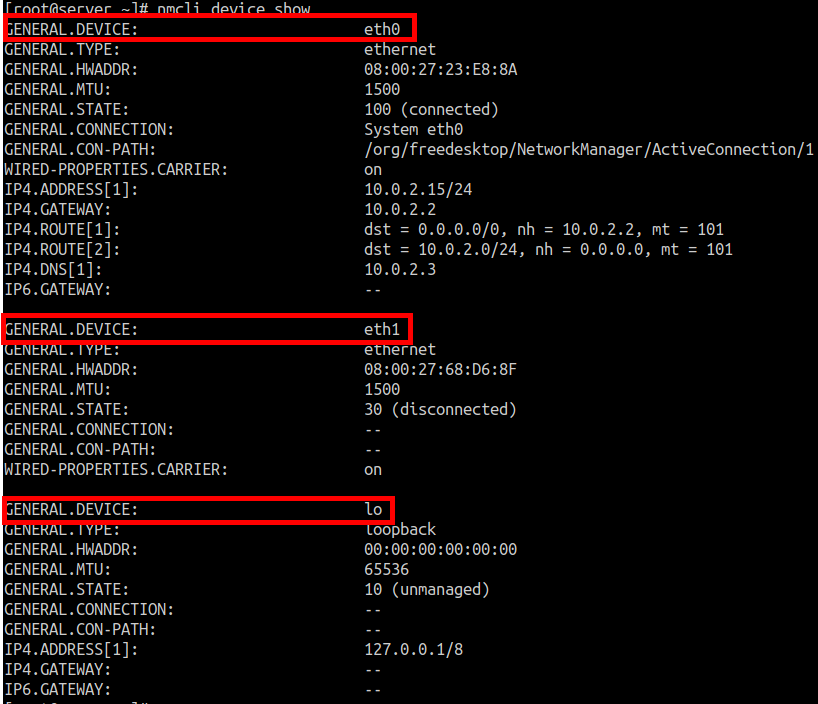
\includegraphics[scale=.35]{content/chapter14/images/cards.png}
			\caption{List of available devices}
			\label{fig:devices}
		\end{figure}		
		\newpage
		\item Display all available connections
		\begin{tcolorbox}[breakable,notitle,boxrule=-0pt,colback=pink,colframe=pink]
			\color{black}
			\fontdimen2\font=9pt
			Syntax: nmcli connection show
			\newline
			or
			\newline
			Syntax: nmcli con show
			\fontdimen2\font=4pt
		\end{tcolorbox}
		Eg:
		\begin{figure}[h!]
			\centering
			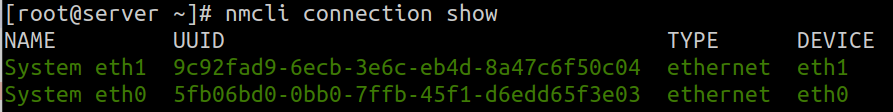
\includegraphics[scale=.35]{content/chapter14/images/show.png}
			\caption{List of available interfaces}
			\label{fig:list}
		\end{figure}		
	
		\bigskip
		\bigskip
		\item Add new connection to an interface:
		\begin{tcolorbox}[breakable,notitle,boxrule=-0pt,colback=pink,colframe=pink]
			\color{black}
			\fontdimen2\font=9pt
			Syntax: nmcli connection add con-name <connection\_name> ifname <interface\_name> type ethernet
			\fontdimen2\font=4pt
		\end{tcolorbox}

		Eg:	
		\begin{tcolorbox}[breakable,notitle,boxrule=-0pt,colback=black,colframe=black]
			\color{green}
			\fontdimen2\font=9pt
			\# nmcli connection add con-name newconnection ifname eth1 type ethernet
			\fontdimen2\font=4pt
		\end{tcolorbox}

		\bigskip
		\bigskip
		\item Provide dynamic IP address (i.e IP from DHCP server) to existing connection:
		\begin{tcolorbox}[breakable,notitle,boxrule=-0pt,colback=pink,colframe=pink]
			\color{black}
			\fontdimen2\font=9pt
			Syntax: nmcli connection modify <connection\_name> ipv4.method auto
			\newline
			\newline
			Syntax: nmcli con mod <connection\_name> ipv4.method auto
			\fontdimen2\font=4pt
		\end{tcolorbox}
		Eg:
		Eg:	
		\begin{tcolorbox}[breakable,notitle,boxrule=-0pt,colback=black,colframe=black]
			\color{green}
			\fontdimen2\font=9pt
			\# nmcli con mod newconnection ipv4.method auto
			\fontdimen2\font=4pt
		\end{tcolorbox}
		

		\bigskip
		\bigskip
		\item Provide IP address to existing connection:
		\begin{tcolorbox}[breakable,notitle,boxrule=-0pt,colback=pink,colframe=pink]
			\color{black}
			\fontdimen2\font=9pt
			Syntax: nmcli connection modify <connection\_name> ipv4.addresses <ip\_address> ipv4.method manual
			\newline
			\newline
			Syntax: nmcli connection up <connection\_name>
			\fontdimen2\font=4pt
		\end{tcolorbox}

		The above command results the changes in below config file:
		\begin{tcolorbox}[breakable,notitle,boxrule=-0pt,colback=pink,colframe=pink]
			\color{black}
			\fontdimen2\font=9pt
			Configuration file:
			\newline
			/etc/sysconfig/network-scripts/ifcfg-<connection\_name>
			\fontdimen2\font=4pt
		\end{tcolorbox}
		
		Eg:	
		\begin{tcolorbox}[breakable,notitle,boxrule=-0pt,colback=black,colframe=black]
			\fontdimen2\font=9pt
			\color{green}
			\# nmcli connection modify newconnection ipv4.addresses 192.168.120.20/24 ipv4.method
			\color{green}
			 manual
			\newline
			\newline
			\color{green}
			\# nmcli connection up newconnection
			\fontdimen2\font=4pt
		\end{tcolorbox}
		
		Notice the changes are reflected in configuration file: \textbf{/etc/sysconfig/network-scripts/ifcfg-newconnection}.
		\begin{figure}[h!]
			\centering
			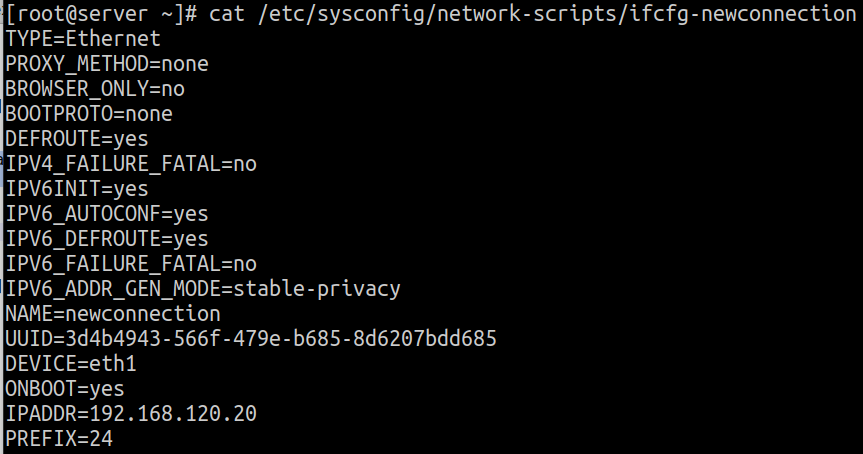
\includegraphics[scale=.35]{content/chapter14/images/networkscript.png}
			\caption{Sample output}
			\label{fig:sample}
		\end{figure}		
	
		\bigskip
		\bigskip
	
		\item Command to set gateway \& dns:
		\begin{tcolorbox}[breakable,notitle,boxrule=-0pt,colback=pink,colframe=pink]
			\color{black}
			\fontdimen2\font=9pt
			Syntax: nmcli connection modify <connection\_name> ipv4.gateway <ip\_address> ipv4.dns <ip\_address>
			\fontdimen2\font=4pt
		\end{tcolorbox}
		Eg:	
		\begin{tcolorbox}[breakable,notitle,boxrule=-0pt,colback=black,colframe=black]
			\color{green}
			\fontdimen2\font=9pt
			\# nmcli connection modify newconnection ipv4.gateway 192.168.122.1 ipv4.dns 192.168.122.254
			\fontdimen2\font=4pt
		\end{tcolorbox}
	
		\bigskip
		\bigskip
		\item Delete connection:
		\begin{tcolorbox}[breakable,notitle,boxrule=-0pt,colback=pink,colframe=pink]
			\color{black}
			\fontdimen2\font=9pt
			Syntax: nmcli connection delete <connection\_name>
			\newline
			or
			\newline
			Syntax: nmcli con del <connection\_name>
			\fontdimen2\font=4pt
		\end{tcolorbox}
		
		Eg:	
		\begin{tcolorbox}[breakable,notitle,boxrule=-0pt,colback=black,colframe=black]
			\color{green}
			\fontdimen2\font=9pt
			\# nmcli con del newconnection
			\fontdimen2\font=4pt
		\end{tcolorbox}
			
	
	
	\end{itemize}
	
	
\end{itemize}




\newpage

\paragraph{Editing interface configuration files}

\begin{itemize}
	\item \textbf{Dynamic configuration}: 
	\begin{itemize}
		\item Create file with name -  \textbf{/etc/sysconfig/network-scripts/ifcfg-<name>} along with below settings:
		\begin{tcolorbox}[breakable,notitle,boxrule=-0pt,colback=black,colframe=black]
			\color{green}
			\fontdimen2\font=9pt
			\# cat /etc/sysconfig/network-scripts/ifcfg-eth0
			\color{white}
			\newline
			NAME="newcon"
			\newline
			TYPE=Ethernet
			\newline
			DEVICE=eth0
			\newline
			ONBOOT=yes
			\newline
			BOOTPROTO=dhcp
			\fontdimen2\font=4pt
		\end{tcolorbox}
		\bigskip
		\bigskip
		\item A description of some of these configuration parameters follows:
		\begin{itemize}
		\item \textbf{TYPE=device\_type}: The type of network interface device.
		\item \textbf{BOOTPROTO=protocol}: Where protocol is one of the following:
		\begin{itemize}
			\item \textbf{none}: No boot-time protocol is used.
			\item \textbf{bootp}: Use BOOTP (bootstrap protocol).
			\item \textbf{dhcp}: Use DHCP (Dynamic Host Configuration Protocol).
		\end{itemize}
		\item \textbf{ONBOOT=answer}: Where answer is one of the following:
		\begin{itemize}
			\item \textbf{yes}: This interface is activated at boot time.
			\item \textbf{no}: This interface is not activated at boot time.
		\end{itemize}
		\item \textbf{DEVICE=interface-name}: Ethernet interface name.
	\end{itemize}
	\bigskip
	\bigskip
	\item Reflect the changes done in the interface configuration file by bringing down the interface and bringing it up again.
	\bigskip
	\begin{tcolorbox}[breakable,notitle,boxrule=-0pt,colback=black,colframe=black]
		\color{green}
		\fontdimen2\font=9pt
		\# nmcli con down eth0
		\newline
		\# nmcli con up eth1
		\fontdimen2\font=4pt
	\end{tcolorbox}		
	\end{itemize}
	
	
	
	\newpage
	
	\item \textbf{Static configuration}:
	\begin{itemize}
		\item Create file with name -  \textbf{/etc/sysconfig/network-scripts/ifcfg-<name>} along with below settings:
		\begin{tcolorbox}[breakable,notitle,boxrule=-0pt,colback=black,colframe=black]
			\color{green}
			\fontdimen2\font=9pt
			\# cat /etc/sysconfig/network-scripts/ifcfg-eth0
			\color{white}
			\newline
			NAME="newcon2"
			\newline
			TYPE=Ethernet
			\newline
			IPADDR0=172.25.4.5
			\newline
			PREFIX0=24
			\newline
			GATEWAY0=172.25.4.254
			\newline
			DEVICE=eth1
			\newline
			ONBOOT=yes
			\newline
			BOOTPROTO=none
			\newline
			DNS0=172.25.254.254
			\fontdimen2\font=4pt
		\end{tcolorbox}
		\bigskip
		\bigskip
		\item A description of some of these configuration parameters follows:
		\begin{itemize}
			\item \textbf{NAME=connection-name}: Connection name for the interface.
			\item \textbf{TYPE=device\_type}: The type of network interface device.
			\item \textbf{IPADDRN=address}: The IPv4 address assigned to the interface
			\item \textbf{PREFIXN=N}: Length of the IPv4 netmask value
			\item \textbf{GATEWAYN=address}: The IPv4 gateway address assigned to the interface. 
			\item \textbf{DNSN=address}: The address of the Domain Name Servers (DNS)

		
			\begin{tcolorbox}[breakable,notitle,boxrule=-0pt,colback=yellow,colframe=yellow]
				\color{black}
				\textbf{Note:} Because an interface can be associated with several combinations of IP address, network mask prefix length, and gateway address, these are numbered starting from 0.
			\end{tcolorbox}

			
			
			\item \textbf{BOOTPROTO=protocol}: Where protocol is one of the following:
			\begin{itemize}
				\item \textbf{none}: No boot-time protocol is used.
				\item \textbf{bootp}: Use BOOTP (bootstrap protocol).
				\item \textbf{dhcp}: Use DHCP (Dynamic Host Configuration Protocol).
			\end{itemize}
			\item \textbf{ONBOOT=answer}: Where answer is one of the following:
			\begin{itemize}
				\item \textbf{yes}: This interface is activated at boot time.
				\item \textbf{no}: This interface is not activated at boot time.
			\end{itemize}
			\item \textbf{DEVICE=interface-name}: Ethernet interface name.
		\end{itemize}
		\bigskip
		\bigskip

		\item Reflect the changes done in the interface configuration file by bringing down the interface and bringing it up again.
		\bigskip
		\begin{tcolorbox}[breakable,notitle,boxrule=-0pt,colback=black,colframe=black]
			\color{green}
			\fontdimen2\font=9pt
			\# nmcli con down eth0
			\newline
			\# nmcli con up eth1
			\fontdimen2\font=4pt
		\end{tcolorbox}
	
		
			
	\end{itemize}
	
	
\end{itemize}

\end{flushleft}
\newpage


